\documentclass[a4paper,11pt]{article}
\usepackage[left=2cm,text={17cm,24cm},top=2cm]{geometry}

\usepackage{times}
\usepackage[czech]{babel}
\usepackage[utf8]{inputenc}
\usepackage[unicode]{hyperref}
\newcommand{\czuv}[1]{\quotedblbase #1\textquotedblleft}
\usepackage{graphicx}
\usepackage{caption}
\usepackage{pdflscape}
\usepackage{graphicx}

\makeatletter

\renewcommand\@pnumwidth{1.5em}   % Ширина колонки с номерами страниц
\newcommand\My@secwidth{2.5ex}    % Ширина колонки с номерами разделов
\newcommand\My@subsecwidth{4.5ex} % Ширина колонки с номерами подразделов

% Стиль заполнения точками
\newcommand{\My@dotfill}{\leavevmode\xleaders\hbox to 1.5mm{\hfil.}\hfill}



\renewcommand*\l@section[2]{%
	\ifnum \c@tocdepth>1
		\setlength\@tempdima{\My@subsecwidth}%
		\setlength\@tempdimb{\My@secwidth}%
		\begingroup
			\parindent \z@ \rightskip \@pnumwidth
			\parfillskip -\@pnumwidth
			\leavevmode
			\advance\leftskip\@tempdima
			\advance\leftskip\@tempdimb
			\hskip -\leftskip
			\hskip \@tempdimb
			#1\nobreak\My@dotfill \nobreak\hb@xt@\@pnumwidth{\hss #2}\par
		\endgroup
	\fi}

\makeatother
%----------------------------------------------------------%
\begin{document}

\begin{titlepage}
    \begin{center}
        \Huge
        \textsc{Vysoké učení technické v~Brně\\
               \huge Fakulta informačních technologií}\\
               
        \vspace{\stretch{0.382}}
        \LARGE
                Databázové systémy\,(IDS) 2022\\
                \Huge Projektová dokumentace\\
                 Projekt č.: 28\\
        \vspace{\stretch{0.618}}
    \end{center}
    
    {\Large \today \hfill
                \begin{tabular}{c}
                Denis Karev\\
                Vladislav Mikheda\\
                \end{tabular}
                }
\end{titlepage}

\begin{center}
{\hypersetup{hidelinks}\tableofcontents}
\end{center}
\newpage

\section{Popis zadání}
Nemocnice\footnote{Zadaní je inspirováno projektem IUS}:\\
Navrhněte Datové model a model případu užití malé nemocnice, který by poskytoval základní údaje o lékařích, sestrách či pacientech, kteří jsou a byli hospitalizováni do nemocnice. IS uchovává informace o všech těchto hospitalizacích, přičemž pacient může ve stejný okamžik hospitalizován pouze na jednom oddělení nemocnice. Při každé hospitalizaci je mu určen jeho ošetřující lékař. Lékaři mohou pracovat na více odděleních zároveň. Na každém oddělení má lékař určitý úvazek, telefon atd., zatímco sestry pracují pouze na jednom oddělení. V rámci pobytu v nemocnici může pacient podstoupit různá vyšetření, která byla provedena na určitém oddělení ve stanoveném čase a provedl ji určitý lékař, který také zapisuje výsledky vyšetření do IS. Dále mu mohou být podávány různé léky, každé podávání léku má určité detaily (kdy se podává, kolikrát apod.).
Zaměřte se i na otázku ochrany dat tak, aby měl každý lékař přístup pouze k potřebným údajům.
\newpage

\section{Model případů užití\,(Use Case Diagram)}
\begin{figure}[h]
\center{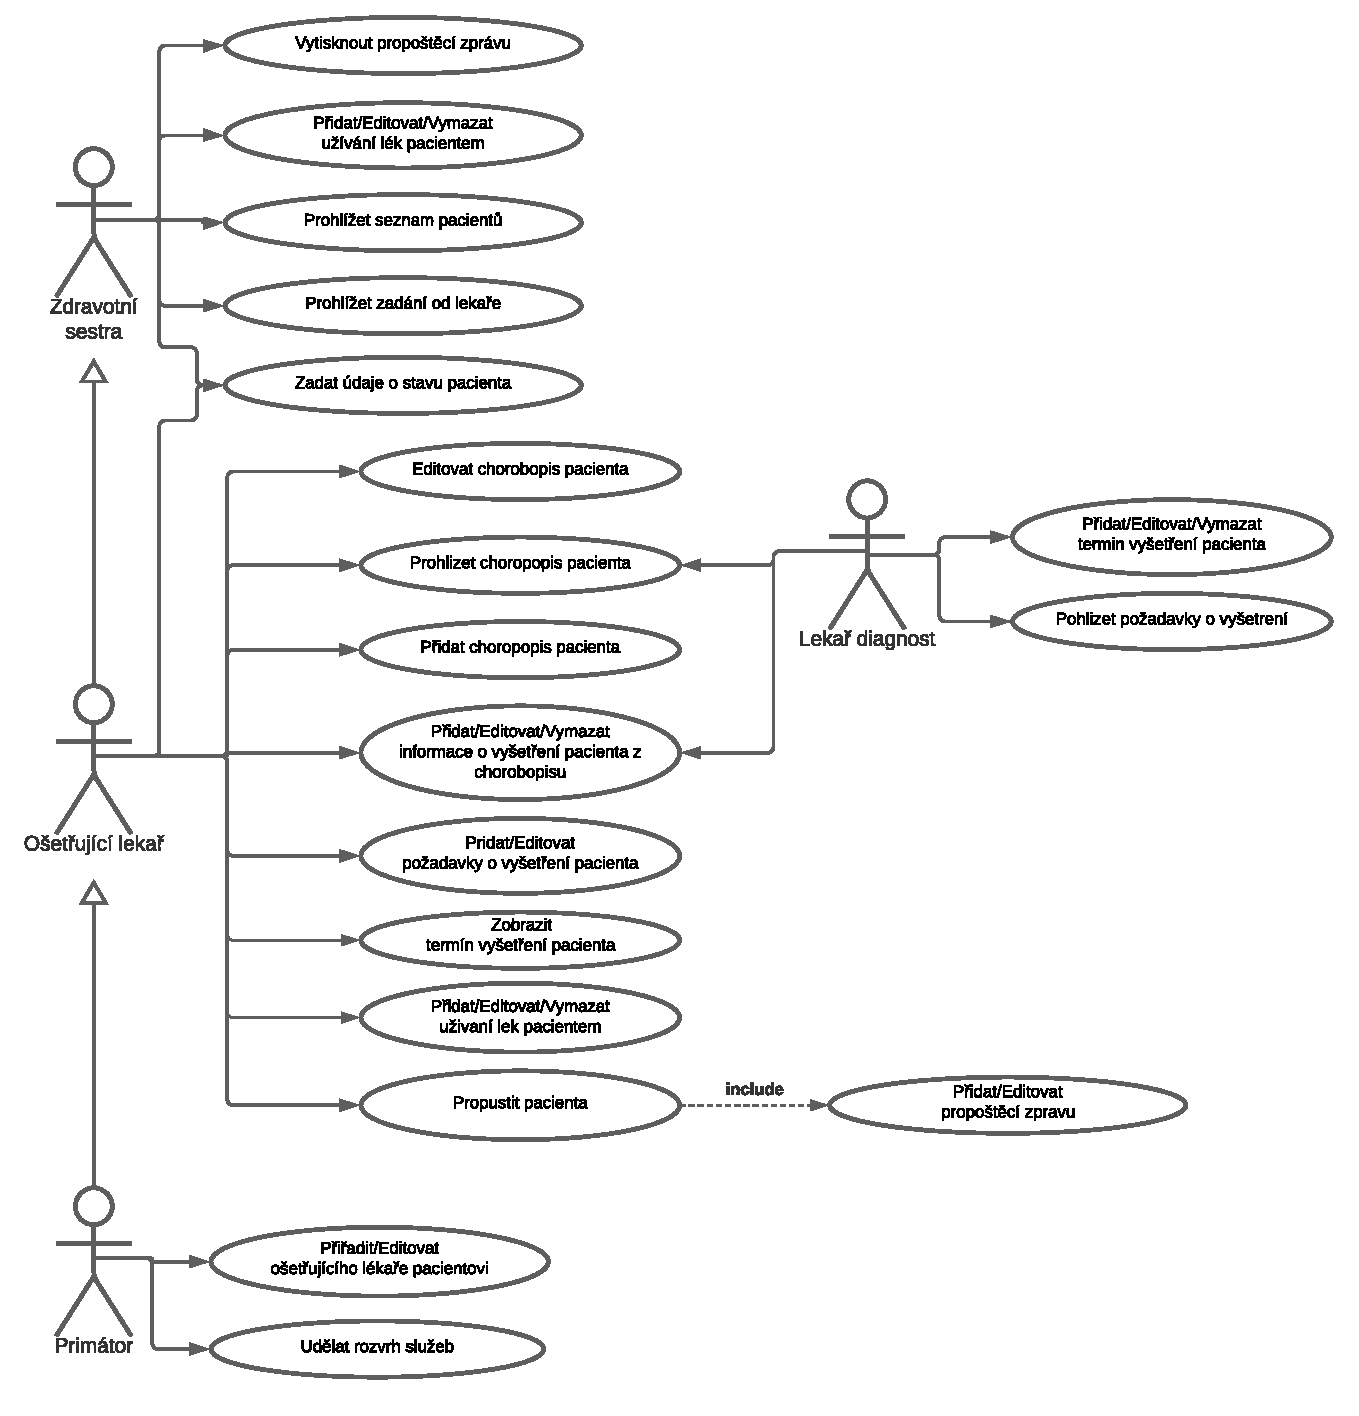
\includegraphics[scale=0.73]{img/useCaseIDS.pdf}}
\caption{Model případů užití}
\label{obrazek:1}
\end{figure}

\newpage
\begin{landscape}
\section{Datový model\,(ERD)}
\begin{figure}[h]
\center{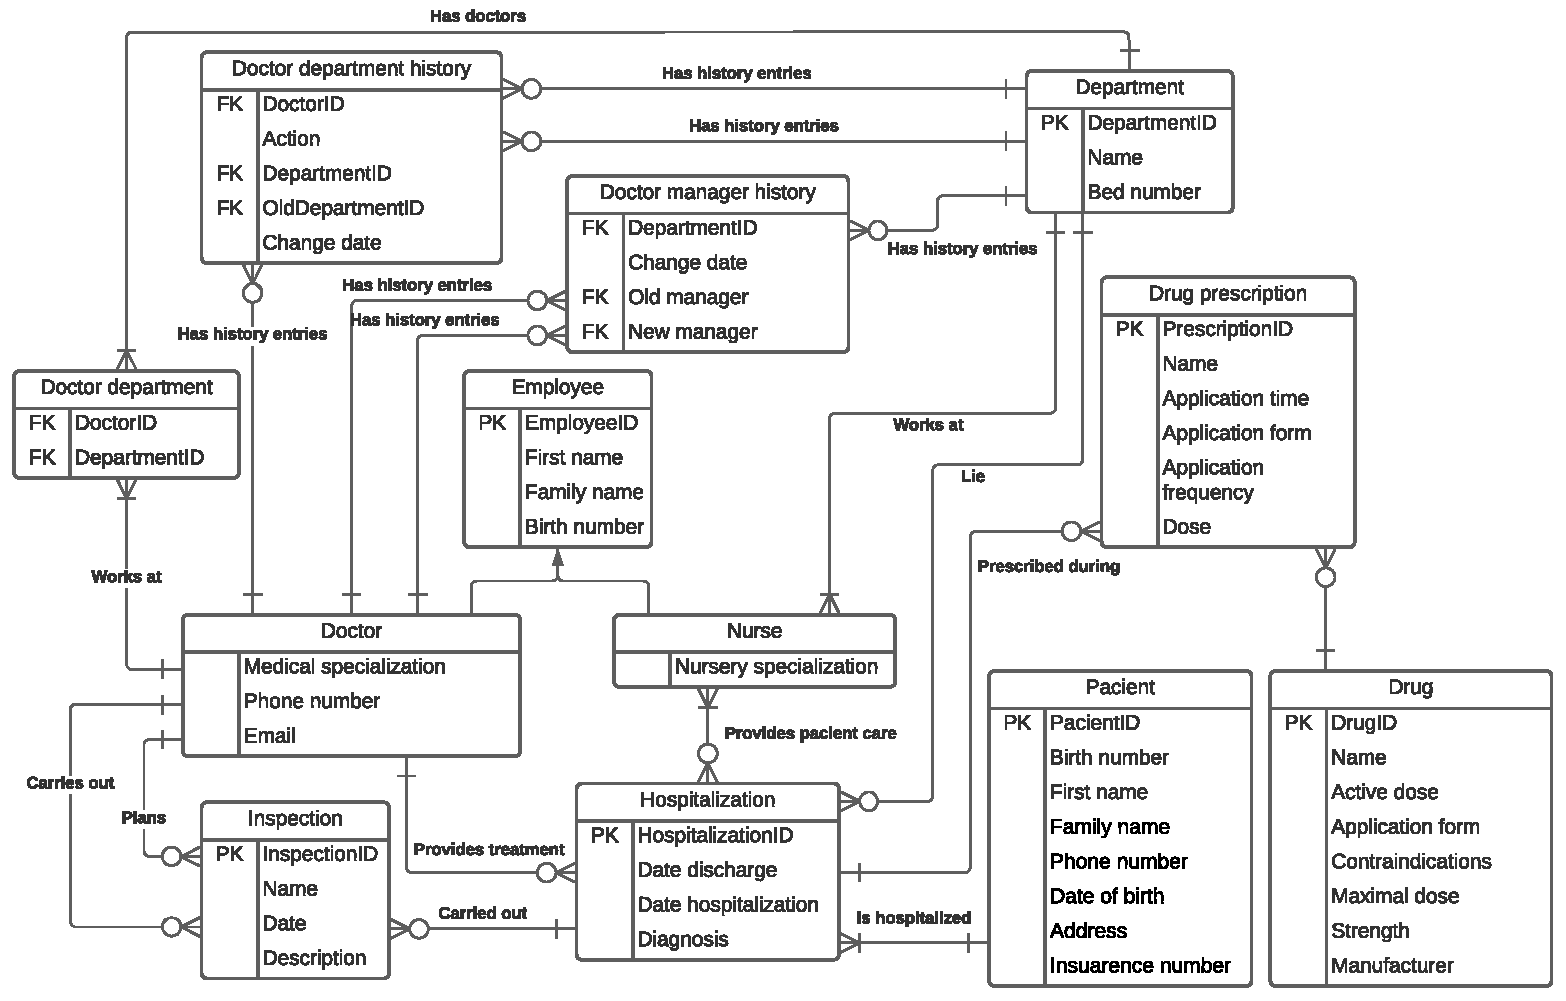
\includegraphics[scale=0.7]{img/erdIDS.pdf}}
\caption{Datové model}
\label{obrazek:2}
\end{figure}
\end{landscape}
\newpage
\section{Realizace generalizace/specializace}
V ERD od entity \texttt{Employee(Personál)} vztahem generalizace/specializace jsou odvedeny dvě entity: \texttt{Doctor(Lékař)}, \texttt{Nurs(Zdravotní sestá)}.\\
\begin{figure}[h!]
\center{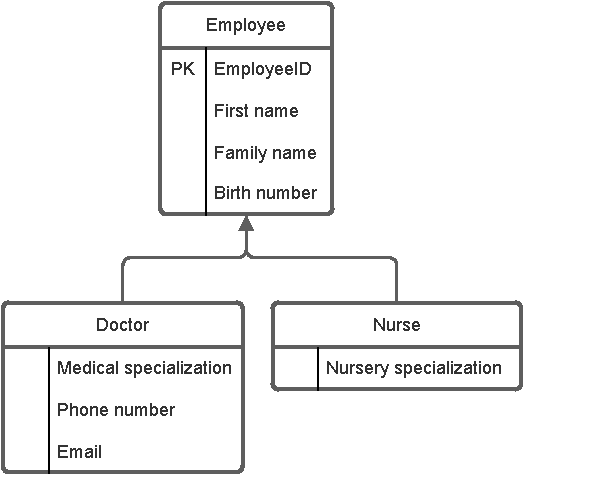
\includegraphics[scale=0.6]{img/spERD.pdf}}
\label{obrazek:3}
\end{figure}\\
Při převodě do tabulky v databázi to bylo vyřešeno
vytvořením tabulky pro nadtyp a také  pro podtypy s primárním klíčem nadtypu. Taková možnost byla zvolena protože potřebujeme dvě různé tabulky pro \texttt{lékaře} a \texttt{zdravotní sestru}. Tabulka \texttt{personál} je využita k ukládání společné informací. Při rozšíření databáze například přidáním tabulky \texttt{maséru} není potřeba nic měnit jen přidat novou tabulku.
\begin{figure}[h!]
\center{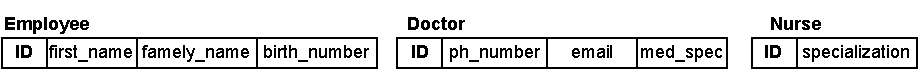
\includegraphics[scale=0.9]{img/spectable.pdf}}
\label{obrazek:3}
\end{figure}\\

\section{Triggery}
Byly vytvořeny dva triggery: \texttt{DEPARTMENT\_MANAGER\_HISTORY\_T} a \texttt{DOCTOR\_DEPARTMENT\_HISTORY}.
Tyto triggery jsou určeny pro logging některých změn v tabulkách. \\

\texttt{DEPARTMENT\_MANAGER\_HISTORY\_T} se vyvolá po změně \texttt{MANAGER\_ID} v tabulce \texttt{DEPARTMENTS}. Tento trigger uloží zkratku oddělení, čas změny, ID starého a nového manažera oddělení do tabulky\\ \texttt{DEPARTMENT\_MANAGER\_HISTORY}. \\

Druhý trigger se aktivuje po přidaní nových dát, změně zkratky oddělení nebo mazaní dát z tabulky \\ \texttt{DOCTORS\_DEPARTMENTS}. Tento trigger využije několik proměnných, protože obsah \texttt{:NEW} a \texttt{:OLD} se mění v závislosti na typu operace. Na konci \texttt{DOCTOR\_DEPARTMENT\_HISTORY} vkládá nový záznam do tabulky \texttt{DOCTOR\_DEPARTMENT\_HISTORY}.

\section{Procedury}
Byly vytvořeny dvě procedury: \texttt{CREATE\_EMPLOYEE} a \texttt{ASSIGN\_DOCTORS}. \\
Procedura \texttt{CREATE\_EMPLOYEE} má následující IN parametry:
\begin{enumerate}
    \item \texttt{IN\_IS\_DOCTOR} - \texttt{BOOLEAN}, je-li nový zaměstnanec doktorem.
    \item \texttt{IN\_BIRTH\_NUMBER} - rodné číslo.
    \item \texttt{IN\_FIRST\_NAME} - jmeno.
    \item \texttt{IN\_FAMILY\_NAME} - příjmení.
    \item \texttt{IN\_SPECIALIZATION} - \texttt{VARCHAR}, specializace.
    \item \texttt{IN\_DEPARTMENT} - zkrátka oddělení.
    \item \texttt{IN\_PHONE\_NUMBER} - telefonní číslo, je volitelným parametrem. 
    \item \texttt{IN\_EMAIL} - email, je volitelným parametrem.
\end{enumerate}
Tato procedura na začátku vytvoří nový záznam v tabulce \texttt{EMPLOYEES}. Potom v závislosti na typu zaměstnance vytvoří nové záznamy v příslušných tabulkách. \\

Procedura \texttt{ASSIGN\_DOCTORS} nemá žádné parametry. Tato procedura přiřadí každé hospitalizace bez doktoru (tj. \texttt{DOCTOR\_ID = NULL}) lékaře s příslušného oddělení. Procedura používá kurzor, který odkazuje na hospitalizace bez doktorů. Pro každý záznam z kurzoru, \texttt{ASSIGN\_DOCTORS} vybere náhodného lékaře (pro náhodný vyber se používá \texttt{ORDER BY DBMS\_RANDOM.RANDOM()}) a přiřadí ho. 

\section{Index, Explain Plan}
Indexy mohou být nastaveny za účelem zrychlení provádění konkrétního dotazu.
Indexy je potřeba přidávat ne na prázdnou tabulku, ale již s nějakými daty, je lepší, když jsou zřídka aktualizovány.
Pro indexaci byl zvolen dotaz \texttt{množství různých léků, které pacienti potřebují.}
Pro zjištění jak se dotaz vykonává využijeme \texttt{Explain Plan}
\begin{figure}[h!]
\center{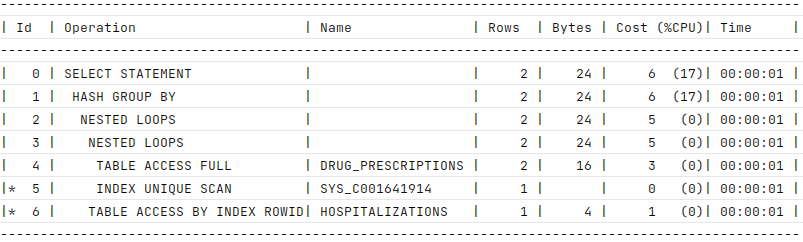
\includegraphics[scale=0.65]{img/DB1.png}}
\label{obrazek:4}
\end{figure}\\
Z plánu lze vidět že jde zpracovaní \texttt{select} dotazů a na začátku bude provedeno grupování položek a pak bude prováděn Procházení každé položky v tabulce \texttt{drug\_prescriptions}, a lze vidět že byly využity indexy které samostatné přidala databáze, pomocí nich je provedeno pouze procházení stromu, dál už bude využit ukazatel na údaje v tabulce.\\
Pro zrychlení dotazu byly zvoleny 2 indexy, první pro sloupce \texttt{date\_disch,id} v tabulce \texttt{hospitalization}, druhý pro \texttt{ABBREVIATION,id\_hosp} v tabulce \texttt{drug\_prescriptions}.\\
\begin{figure}[h!]
\center{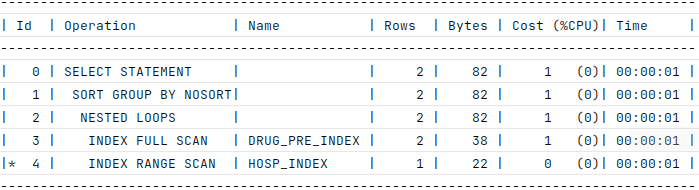
\includegraphics[scale=0.7]{img/DB2.png}}
\label{obrazek:4}
\end{figure}\\
Lze vidět že procházení tabulek s využitím indexu zrychli dotazovaní.
\section{Materializovaný pohled}
Byly vytvořeny dva materializovaných pohledy, byly využity \texttt{BUILD IMMEDIATE} co naplní pohled při vytváření, pro první bylo vyžito \texttt{REFRESH COMPLETE ON DEMAND} aktualizuje se přepočítáním definujícího dotazu materializovaného pohledu, pro aktualizace je využit postup \texttt{DBMS\_MVIEW.REFRESH}.
V druhém materializovaném pohledu je využito \texttt{REFRESH COMPLETE ON COMMIT}. Což vyžaduje využití \texttt{COMMIT}, co ukončí transakci a
uloží změny.
\end{document}


% V ERD od entity \texttt(Employee(Personál)) vztahem generalizace/specializace jsou odvedeny dvě entity: \texttt(Doctor(Lékař)),\texttt(Nurs(Zdravotní sestá)).
% \section{Popis Datového modelu}
% \begin{itemize}
%     \item {\bf Entita Pacient (Pacient)} reprezentuje všechny pacienty, kteří jsou nebo byli někdy hospitalizovány.
%     \begin{itemize}
%         \item Pacient muže mít několik hospitalizací během svého života.
%     \end{itemize}

%     \item {\bf Entita Hospitalization (Hospitalizace)} reprezentuje jednorázový pobyt           pacienta v nemocnici.
%     \begin{itemize}
%         \item Může obsahovat jen jednoho pacienta.
%         \item Při hospitalizaci mohou být prováděny nějaká ošetření.
%         \item Ke každé hospitalizaci je přiřazen jeden lékař který léčí.
%         \item Ke každé hospitalizaci je předepsaná sestřička která se stará o pacienta, může být i několik podle různých potřeb.
%         \item Ke každé hospitalizaci může být předepsán nějaký lék nebo žádný, člověk může být hospitalizován jen za účelem vyšetření. 
%     \end{itemize}

%      \item {\bf Entita Inspection (Vyšetřeni)} Popisuje jednotlivá vyšetření při jednotlivé hospitalizace.
%     \begin{itemize}
%         \item Může být prováděno jen při hospitalizaci.
%         \item Je naplánováno ošetřujícím lékařem.
%     \end{itemize}
    
%     \item {\bf Entita Drug prescription (Předpis na léky)} reprezentuje jednotlivé léky které budou předepsané pacientovi při jednotlivé hospitalizaci.
%     \begin{itemize}
%         \item Může obsahovat jen jeden lék
%         \item Předpis na léky je předepsán pro jednu určitou hospitalizace, protože záleží na diagnóze a t.d.
%     \end{itemize}
    
%     \item {\bf Entita Drug (Lék)} popisuje vlastnosti jednoho léku
%     \begin{itemize}
%         \item Může být využít pro několik nebo pro žádný        předpis
%     \end{itemize}
    
%     \item {\bf Entita Employee (Personál)} reprezentuje personál který pracuje v nemocnici a od něj vztahem generalizace/specializace jsou odvedeny dvě entity: {\bf lékař} a {\bf zdravotní šestá}.
    
%     \item {\bf Entita Doctor (Lékař)} reprezentuje lékaře kteří pracují v nemocnici (ošetřovací lékař, lékař diagnost, primátor).
%     \begin{itemize}
%         \item Jeden lékař se najednou může zúčastnit několika hospitalizacích nebo žádné.
%         \item Může si plánovat vyšetření.
%         \item Může vyšetření provádět.
%         \item Může pracovat zároveň v několika odděleních a v diagramu je to popsány pomocí vazební tabulky.
%     \end{itemize}
    
%     \item {\bf Entita Nurse (Zdravotní setra)} reprezentuje zdravotních sester které pracují v nemocnici.
%     \begin{itemize}
%         \item Může se najednou zúčastnit několika hospitalizací nebo žádné.
%         \item Může být přiřazena k několika hospitalizacím nebo k žádné.
%         \item Může pracovat jen v jednom oddělení
%     \end{itemize}
    
    
%     \item {\bf Entita Department (Oddělení)} reprezentuje oddělení v nemocnici.
%     \begin{itemize}
%         \item V odděleni musí pracovat alespoň jedna sestra ale může i víc.
%         \item V oddělení je nutné aby pracoval alespoň jeden lékař.
%     \end{itemize}

% \end{itemize}